% ######################################################################################################################
%         Introduction
% ######################################################################################################################

\chapter{Introduction}
\label{ch:Introduction}

% ######################################################################################################################
%         Background and Motivation
% ######################################################################################################################

\section{Background and Motivation}
\label{ch:Introduction:sec:Motivation}

The concept of evolution is one of the cornerstones of modern biology \cite{Dobzhansky1973}.
% \secref{ch:Foundations:sec:EvolutionGenetics}
All life on earth descends from a common ancestor and continuously evolves and adapts over generations,
which leads to a diversification of biological species.
The resulting branching pattern of the evolutionary relationships between species
is the key for unraveling many biological questions,
ranging from paleontology \cite{Schaeffer1972} to medicine \cite{Hartfield2014}. %and bio-technology.
These evolutionary relationships are described by \emph{phylogenetic trees}
(\secref{ch:Foundations:sec:TreeOfLife}),
which are important in both fundamental \cite{Misof2014,Jarvis2014,Zanne2014} and
applied research \cite{Futuyma1995,Hendry2011,Schwartz2017}.

Characteristics and traits of biological species are inherited via their DNA
(\secref{ch:Foundations:sec:EvolutionGenetics}).
DNA data is hence often used for inferring a phylogenetic tree for a set of species
(\secref{ch:Foundations:sec:MLTreeInference}).
In order to conduct such analyses, the DNA has to be sequenced,
that is, it has to be ``read'' into some human-accessible format,
typically in form of a sequence of characters
(\secref{ch:Foundations:sec:SequenceAnalysis}).
In recent decades, the throughput of sequencing technologies has increased substantially,
while at the same time, the cost has decreased faster than Moore's law,
as shown in \figref{fig:sequencing_costs}.
Currently, the sequencing capacity doubles roughly every seven months \cite{Stephens2015}.
This lead to a ``tsunami'' of sequence data,
which constitutes a major challenge for conducting computational analyses of these data.
% computational biology

\begin{figure}[hbt]
    \centering
    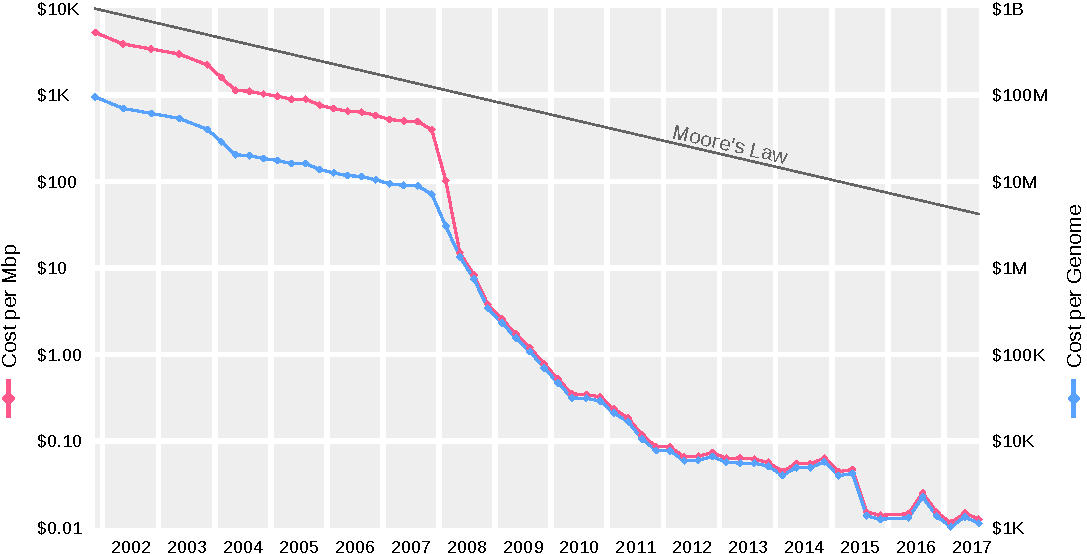
\includegraphics[width=\linewidth]{sequencing_costs.pdf}
    \caption[Sequencing costs per Mbp and per genome]{
        \textbf{Sequencing costs per Mbp and per genome.}
        The cost for DNA sequencing have decreased substantially in the past 15 years.
        The Figure shows the cost per mega-basepair (Mbp) of DNA (red line, left y-axis)
        as well as the cost per human-sized genome of $\approx$\,\num{3}\,Gbp (blue line, right y-axis).
        A basepair represents one character in the DNA.
        Note the logarithmic scaling of the y-axes.
        For comparison, Moore's law \cite{Moore1965} is shown.
        The particularly steep decrease in the beginning of 2008 is caused by
        the adoption of novel (high-throughput) sequencing technologies in sequencing centers,
        see \secref{ch:Foundations:sec:SequenceAnalysis:sub:GenomeSequencing}.
        Source: Image based on data from \cite{Wetterstrand2018}.
%         \url{https://www.genome.gov/sequencingcosts/}
%         \url{https://www.genome.gov/sequencingcostsdata/}
    }
    \label{fig:sequencing_costs}
\end{figure}

In particular, these high-throughout technologies allow to directly sequence DNA contained in samples
that have been extracted from environments such as water, soil, or the human gut.
This results in so-called \emph{metagenomic} sequences,
that is, anonymous DNA sequences from the (microbial) organisms that were present in the environmental sample.
A key question in the analysis of such data is to determine the evolutionary relationships of the sequences.
While these DNA sequences can hypothetically be used to infer phylogenetic trees from scratch,
this approach is limited by several theoretical and practical difficulties:
For instance, typical metagenomic samples contain too many, and too short, sequences
for a feasible and reliable tree inference \cite{Matsen2010,Janssen2018}.

One approach to tackle this issue is to deploy so-called \emph{phylogenetic placement} \cite{Matsen2010,Berger2011}
of metagenomic sequences on a given phylogenetic tree (\secref{ch:Foundations:sec:PhylogeneticPlacement}).
Phylogenetic placement methods classify a set of \emph{query sequences}
into the context of known evolutionary relationships, provided in form of a \emph{phylogenetic reference tree}.
While this information already represents biological knowledge per se,
it can also be used for further downstream analyses \cite{Matsen2011a}.
Although such phylogeny-aware methods offer large potential for sequence data analysis and interpretation,
the research in this field is relatively recent and only a few such analysis methods have been developed so far.

An important task prior to conducting phylogenetic placement of metagenomic sequences is to obtain a suitable
phylogenetic reference tree that captures the biological diversity of the species to be placed.
The assembly of a set of reference sequences from biological databases that can be used to infer such a tree
is typically a manual process, and hence both labor-intensive and potentially error-prone.
This might detain researchers from employing phylogenetic placement in the first place,
and make them resort to simpler methods based on sequence similarity/identity instead.

Furthermore, while the existing downstream analysis methods for phylogenetic placement
(introduced in \secref{ch:Foundations:sec:PhylogeneticPlacement:sub:ExistingMethods})
allow for in-depth interpretation and visualization of the data,
they were not developed with a particular focus on large-scale studies
comprising thousands of environmental samples and billions of sequences.
For large datasets, these methods might provide too much detail,
making it hard to interpret results, to detect patterns or clusters in the data,
and to discover correlations with per-sample meta-data.

Lastly, the problem of scalability on large datasets does not only affect the methods themselves.
Because of the ever growing amount of sequence data,
scalability is becoming an issue for the software pipelines as well.
State-of-the-art phylogenetic placement implementations can process billions of sequences within a few hours \cite{Barbera2018}.
Methods for handling and analyzing the data, in particular phylogenetic placement data,
hence require efficient and scalable software implementations.

% ######################################################################################################################
%         Objective and Contribution
% ######################################################################################################################

% \section{Objective and Contribution}
% \label{ch:Introduction:sec:ObjectiveContribution}

\section{Scientific Contribution}
\label{ch:Introduction:sec:ContributionOverview}

This thesis makes several contributions to the field of computational phylogenetics,
specifically regarding phylogenetic placements as well as analyzing and visualizing the resulting data.
In particular, we introduce multiple novel methods to overcome the issues and limitations explained above.
We described the methods in two already peer-reviewed open-access publications \cite{Czech2018-phat,Czech2019-analysis},
and made their data and scripts available at \url{http://github.com/lczech/placement-methods-paper}.
More details on the contribution of each method to the research community are provided in the respective chapters.

Apart from the two publications on which this thesis is based,
we published a review on several software tools for visualizing phylogenetic trees \cite{Czech2017-tree-viewers}.
In this publication, we investigated whether certain types of per-branch and per-node meta-data of phylogenetic trees
were correctly displayed in \num{20} distinct tree visualization tools.
% particularly when first modifying the tree topology.
We found that most of the tested tools exhibited problems or undocumented behavior and
did not properly support the \fileformat{Newick} file format for phylogenetic trees.
We also showed that this has already affected trees published in peer-reviewed journals.
At the time of its publication, our review had already led to improvements in eight of the twenty tested tools.

In addition to these theoretical projects, we also contributed to several empirical data analysis studies
by conducting established analyses as well as testing prototypes of our novel methods presented here.
In particular, we ran the phylogenetic analyses for a study of \num{154} locations
in neotropical rainforest soils, which was published in \textit{Nature Ecology \& Evolution} \cite{Mahe2017}.
The study found that the microbial diversity in these soils is dominated by hyper-diverse protistic parasites.
For this project, we developed prototypes of our multilevel placement approach
(\secref{ch:AutomaticTrees:sec:Methods:sub:MultilevelPlacement})
as well as of some visualization techniques (\secref{ch:Visualization:sec:Motivation}).

Further data analysis studies that we contributed to include the 1KITE project \cite{Misof2014} (\url{http://1kite.org}),
for which we conducted phylogenetic tree reconstructions for a diverse set of \num{1500} insects,
as well as a study of \taxonname{Microsopirida} and \taxonname{Cryptomycota} \cite{Bass2018a},
to which we contributed phylogenetic placement analyses
in order to resolve some branches in the phylogenetic tree of these groups of microbial \taxonname{Eukaryotes}.
An ongoing large-scale endeavor is the UniEuk project \cite{Berney2017},
which aims to offer a unified reference database for the \taxonname{Eukaryotes}.
For UniEuk, we provided consultancy and helped in planning workflows and pipelines.
Furthermore, for its sub-project EukBank,
we conducted preliminary phylogenetic analyses of their entire metagenomic database as a showcase for other researchers.
In a current empirical data analysis project,
we develop tools for analyzing a dataset of microbial \taxonname{Eukaryotes} \cite{Jamy2019a}.
The goal is to show that novel sequencing technologies that yield longer sequences per run
can improve taxonomic and phylogenetic analyses compared to other sequencing technologies.
Lastly, we are currently working on an empirical dataset of \taxonname{Dinoflagellates},
for which we also conducted phylogenetic placement analyses.

% In the course of developing our novel methods, we implemented them in \texttt{C++11},
We implemented all of our novel methods in \texttt{C++11},
and provide the resulting code in our open-source library \toolname{genesis} (\url{https://github.com/lczech/genesis}).
Apart from the novel methods, the library provides efficient re-implementations of existing methods,
for example the Edge PCA and Squash Clustering methods of \toolname{guppy} \cite{Matsen2010},
which we introduce in \secref{ch:Foundations:sec:PhylogeneticPlacement:sub:ExistingMethods}.
Our implementations are faster than the original one by orders of magnitude \cite{Czech2018-phat}.
Furthermore, the library also offers a multitude of data structures and functions for working with
phylogenetic placements, genetic sequences, phylogenetic trees, taxonomies, and many other data types.
It also provides a plethora of auxiliary functions for tasks such as visualization, statistical evaluation, and data storage.
Moreover, in order to also offer a user-friendly command line interface for the most important novel and established methods,
we developed the open-source tool \toolname{gappa} (\url{https://github.com/lczech/gappa}),
which stands for ``Genesis Applications for Phylogenetic Placement Analysis''.
It is intended for researchers who desire to conduct analyses using our methods.
It internally uses the \toolname{genesis} library for its computations.
For details on the software implementations, see \appref{ch:PipelineImplementation}.
We also published an application note \cite{Czech2019-genesis-gappa},
which describes \toolname{genesis} and \toolname{gappa} in detail,
and evaluates their runtime and memory requirements in comparison to analoguous software.

Moreover, we contributed to several other open-source bioinformatics software projects.
We helped to develop an efficient approach for merging so-called \emph{paired-end reads}
and provided SIMD (single instruction, multiple data) implementations using \texttt{SSE} and \texttt{AVX} instructions
to accelerate the merging algorithm \cite{Flouri2017}.
Again for acceleration, we implemented a custom \texttt{\acs{MPI}} wrapper for \toolname{PaPaRa 2.0} \cite{Berger2011a,Berger2012},
which we made available at \url{https://github.com/lczech/papara_nt}.
\toolname{PaPaRa} is a tool for aligning query sequences to a given reference alignment and phylogenetic tree,
which is a necessary pre-processing step for phylogenetic placement.
During the development of the recent high-performance re-implementation of the phylogenetic placement algorithm
in \toolname{EPA-ng} \cite{Barbera2018}, we provided support for software design decisions and implementation details.
Also, our \toolname{genesis} library was used and extended for this project.
We moreover contributed to the implementation and acceleration of a novel quartet-based method to accurately and robustly
measure incongruence between phylogenetic trees \cite{Zhou2017};
the \toolname{genesis} library was used for this project as well.
Furthermore, we contributed code to the sequence clustering tool \toolname{swarm} \cite{Mahe2014,Mahe2015},
which we briefly introduce in \secref{ch:Foundations:sec:SequenceAnalysis:sub:OTUs}.
Our code was the basis for accelerating the runtime of the tool by factors of up to \num{20}-fold,
while at the same time significantly reducing its memory requirements.
These improvements will be part of the upcoming version~3 of \toolname{swarm}.
Lastly, we are currently working on \toolname{scrapp},
a pipeline that combines several tools developed in our lab, such as
\toolname{EPA-ng} \cite{Barbera2018}, \toolname{ParGenes} \cite{Morel2019}, and \toolname{mPTP} \cite{Kapli2017},
in order to estimate the species diversity of metagenomic sequence samples based on phylogenetic placement data;
see also \chpref{ch:ConclusionFutureDirections}.

% A full list of our publications is also available in \appref{ch:Publications}.
% tree clustering workshop?

% ######################################################################################################################
%         Structure and Overview
% ######################################################################################################################

\section{Structure and Overview}
\label{ch:Introduction:sec:StructureOverview}

The remainder of this thesis is structured as follows.
Initially, we introduce the general concepts and existing methods
of computational phylogenetics and phylogenetic placement (\chpref{ch:Foundations}).
In subsequent chapters, we describe our novel methods for conducting and analyzing phylogenetic placements:
Firstly, we describe an automated approach for obtaining suitable reference trees for phylogenetic placement,
as well as pre-processing pipelines to accelerate and enable
phylogenetic placement of large metagenomic datasets (\chpref{ch:AutomaticTrees}).
Secondly, we introduce methods to visualize such large datasets
in order to detect patterns within the data and correlations with per-sample meta-data (\chpref{ch:Visualization}).
Then, we present an approach for clustering metagenomic samples (\chpref{ch:Clustering}),
by measuring similarity between samples in terms of the species diversity they contain.
In between, we describe an adaptation of a novel type of data representation
to phylogenetic placement data (\chpref{ch:Balances}).
Lastly, we present an adaptation of a recent method called Phylofactorization
to phylogenetic placement data (\chpref{ch:Factorization}),
which allows to find parts of a given reference tree
that are meaningful with respect to meta-data features collected per environmental sample.
Finally, we conclude and discuss potential directions of future work (\chpref{ch:ConclusionFutureDirections}).
We furthermore provide additional supporting information (\appref{ch:SupportingInformation}),
an overview of the empirical datasets used for our evaluations and their pre-processing (\appref{ch:EmpiricalDatasets}),
as well as some information on our software implementation (\appref{ch:PipelineImplementation}).

% Most of the above chapters are derived either fully or in part from parts of two of our publications,
% namely \citeay{Czech2018-phat} and \citeay{Czech2019-analysis}.
% Each chapter states the contributions and other relevant background information in its beginning;
% we here briefly summarize these.

% this thesis is mainly derived from two publications.
% we mark each chapter with the respective publicaation that it is based on.
% here we briefly summarize the contributes to each publication, in order to avoid repeating this information later.


% \todo{search for all abbreviations used and add them to the acro list. also, check Pierre's MA, and Alexey's and Andre's Diss for needed acronyms!}
% 
% \todo{list of acronyms!} see andre, add MB/GB, PCA, BV, TO, HMP, etc
% 
% \todo{for re-calculated figures, add the author name. instead of saying ``recalc of fig x of [abc]'', say ``recalc of fig x of bla et al [abc]''!}
% 
% \todo{unify spelling of taxa: sometimes, we use lower case bacteria, sometimes upper cased, etc. sometimes eukaryota, somtimes Eukaryotes...}
% 
% \todo{para vs poly phyletic!}
% 
% \todo{make sure to update the bioRxiv preprints to the actual publications! not only here, but everywhere! my papers, quartet, epa, etc}
